\documentclass[conference]{IEEEtran}
\usepackage{cite,amsmath,amssymb,graphicx,booktabs,xcolor,tikz,pgfplots}
\usetikzlibrary{arrows.meta,positioning,fit,calc}
\pgfplotsset{compat=1.18}
% Red placeholders: replace every \tbd{...} with the measured value.
\newcommand{\tbd}[1]{\textcolor{red}{\textbf{[#1]}}}
\newcommand{\name}{\textsc{PhaSched}}

\begin{document}

\title{Late Breaking Results: Round-Phase-Aware Memory Scheduling for Federated Learning Clients}

% Double-blind submission: add authors only in the camera-ready version.
\author{\IEEEauthorblockN{Anonymous Author(s)}
\IEEEauthorblockA{Submitted for double-blind review}}

\maketitle

\begin{abstract}
The main-memory traffic of a federated learning (FL) client follows the round structure of the protocol: the network interface writes the global model into DRAM, the cores read and update it during local training, and the network interface reads the update back out. Existing memory schedulers are unaware of these phases and apply a single policy throughout. We propose \name{}, which exposes a 2-bit round-phase register to the memory controller and uses it to select among lightweight presets of an FR-FCFS scheduler. \name{} needs no per-thread state. Evaluated in DAMOV-SIM on \tbd{N} FL workloads, it reduces round time by \tbd{X\%} and average read latency by \tbd{Y\%} over FR-FCFS.
\end{abstract}

\begin{IEEEkeywords}
federated learning, memory controller, DRAM scheduling, edge computing
\end{IEEEkeywords}

\section{Introduction}
Federated learning (FL) trains a shared model across many clients without moving their data~\cite{fedavg}. In every round a client downloads the global model, trains it on local data and uploads an update. Systems work on FL clients has concentrated on communication cost and on compute heterogeneity~\cite{flscale,flopen}; how a round stresses main memory has received little attention.

We observe that an FL round imposes three distinct and \emph{predictable} traffic patterns on the memory controller (Fig.~\ref{fig:overview}, top):
\begin{itemize}
\item \textbf{Ingress.} The NIC writes the model, tens of megabytes for common vision networks~\cite{resnet}, into DRAM by DMA. The traffic is a sequential, write-only burst.
\item \textbf{Train.} The cores read weights and activations and write gradients and updated weights. Reads dominate and determine progress; writes are not urgent.
\item \textbf{Egress.} The NIC reads the update out of DRAM by DMA. The traffic is a sequential, read-only stream.
\end{itemize}

A conventional controller uses FR-FCFS~\cite{frfcfs} with a fixed write-drain policy. Thread-aware schedulers such as PAR-BS~\cite{parbs}, ATLAS~\cite{atlas}, TCM~\cite{tcm} and BLISS~\cite{bliss} improve fairness and throughput across competing threads, and learning-based controllers~\cite{rlsched} adapt reactively. None of them is told what the application already knows exactly: which phase of the round it is in. As a result the controller toggles between read and write mode at the wrong moments, pays bus-turnaround delays, and interrupts row-hit streaks on streams that are perfectly sequential.

\textbf{Contribution.} We propose \name{}, a phase-aware extension of FR-FCFS in which the FL runtime announces the current round phase to the memory controller, and the controller switches to a preset tuned for that phase. The mechanism costs a 2-bit register and a four-entry preset table, and requires three register writes per round.

\begin{figure}[t]
\centering
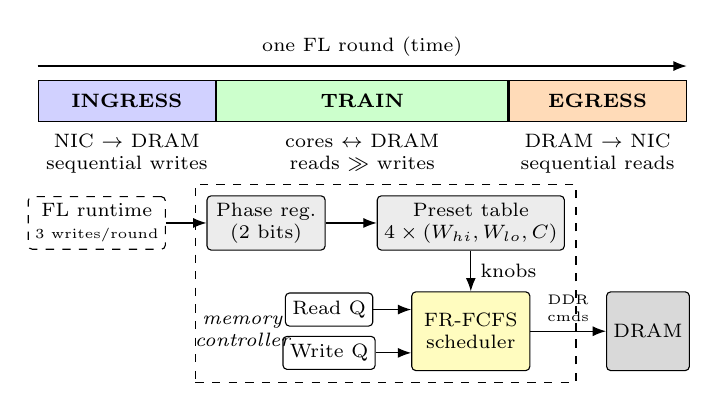
\begin{tikzpicture}[font=\scriptsize,>=Latex,
  ph/.style={draw,minimum height=0.52cm,inner sep=1pt},
  blk/.style={draw,rounded corners=1.5pt,minimum height=0.55cm,align=center,inner sep=2.5pt}]
% ---- round timeline
\node[ph,fill=blue!18,minimum width=2.25cm,anchor=west] (ing) at (-0.75,0) {\textbf{INGRESS}};
\node[ph,fill=green!20,minimum width=3.7cm,right=0pt of ing] (trn) {\textbf{TRAIN}};
\node[ph,fill=orange!28,minimum width=2.25cm,right=0pt of trn] (egr) {\textbf{EGRESS}};
\node[below=1pt of ing,align=center] (ingl) {NIC $\rightarrow$ DRAM\\sequential writes};
\node[below=1pt of trn,align=center] (trnl) {cores $\leftrightarrow$ DRAM\\reads $\gg$ writes};
\node[below=1pt of egr,align=center] (egrl) {DRAM $\rightarrow$ NIC\\sequential reads};
\draw[->] ([yshift=5pt]ing.north west) -- node[above,pos=0.5]{one FL round (time)} ([yshift=5pt]egr.north east);
% ---- controller
\node[blk,dashed,minimum width=1.45cm] (rt) at (0,-1.55) {FL runtime\\{\tiny 3 writes/round}};
\node[blk,fill=gray!15,minimum width=1.5cm] (reg) at (2.15,-1.55) {Phase reg.\\(2 bits)};
\node[blk,fill=gray!15,minimum width=2.3cm] (tab) at (4.75,-1.55) {Preset table\\$4\times(W_{hi},W_{lo},C)$};
\node[blk,minimum width=1.05cm,minimum height=0.42cm] (rq) at (2.95,-2.65) {Read Q};
\node[blk,minimum width=1.05cm,minimum height=0.42cm] (wq) at (2.95,-3.2) {Write Q};
\node[blk,fill=yellow!25,minimum width=1.5cm,minimum height=1.0cm] (sch) at (4.75,-2.925) {FR-FCFS\\scheduler};
\node[blk,fill=gray!30,minimum width=0.9cm,minimum height=1.0cm] (dram) at (7.0,-2.925) {DRAM};
\draw[->] (rt) -- (reg);
\draw[->] (reg) -- (tab);
\draw[->] (tab) -- node[right]{knobs} (sch);
\draw[->] (rq.east) -- (rq.east -| sch.west);
\draw[->] (wq.east) -- (wq.east -| sch.west);
\draw[->] (sch) -- node[above,font=\tiny,align=center]{DDR\\cmds} (dram);
\node[draw,dashed,inner sep=4pt,fit=(reg)(tab)(sch)(rq)(wq)] (mc) {};
\node[align=center,font=\scriptsize\itshape] at (1.85,-2.925) {memory\\controller};
\end{tikzpicture}
\caption{Top: memory traffic of one FL round on a client. Bottom: \name{}. The FL runtime writes the current phase; the phase selects the write-drain watermarks $W_{hi}$, $W_{lo}$ and the row-hit streak cap $C$ used by an otherwise unmodified FR-FCFS scheduler.}
\label{fig:overview}
\end{figure}

\section{\name{}}
\subsection{Phase Interface}
The controller holds a register $\textsc{phase}\in\{\textsc{idle},\textsc{ingress},\textsc{train},\textsc{egress}\}$. The FL runtime updates it through a privileged register write at the three points where the round changes character: before it starts receiving the model, before it starts local training, and before it starts sending the update. These points already exist as distinct calls in FL frameworks, so no application restructuring is needed. When the register holds \textsc{idle}, the controller behaves exactly as the baseline, so non-FL software is unaffected.

\subsection{Phase Presets}
\name{} does not introduce a new scheduling algorithm. It re-tunes three knobs that an FR-FCFS controller already has: the high and low write-queue watermarks $W_{hi}$ and $W_{lo}$, which decide when the controller enters and leaves write-drain mode, and the cap $C$ on consecutive row hits served before an older request to another row is considered. Table~\ref{tab:presets} lists the presets.

\begin{table}[t]
\centering
\caption{Phase presets of \name{}}
\label{tab:presets}
\footnotesize
\begin{tabular}{@{}llll@{}}
\toprule
Phase & Write drain & Row-hit cap $C$ & Intent \\
\midrule
\textsc{idle} & baseline & baseline & unchanged behaviour \\
\textsc{ingress} & eager: enter when & unlimited & long write bursts, \\
 & queue non-empty & & one activation per row \\
\textsc{train} & lazy: drain when & baseline & reads never wait \\
 & reads idle or $W_{hi}$ & & behind writes \\
\textsc{egress} & only at $W_{hi}$ & raised & uninterrupted \\
 & & & read stream \\
\bottomrule
\end{tabular}
\end{table}

\textbf{Ingress} favours writes. The controller enters write mode as soon as the write queue is non-empty and stays there until it is empty. Because the DMA stream fills rows in order, lifting the row-hit cap lets each row be activated once and written completely, and the number of write-to-read turnarounds falls to nearly zero.

\textbf{Train} favours reads. Writes of gradients and weights are buffered and drained when the read queue is empty or the write queue reaches $W_{hi}$. The cap stays at its baseline value to preserve fairness among training threads.

\textbf{Egress} pins the controller in read mode with a raised cap, so the sequential read stream of the NIC is served in long row-hit runs; residual writes are drained only at $W_{hi}$.

\textbf{Starvation guard.} In every phase a request that has waited longer than $T_{max}$ is served next. This bounds the delay of any traffic that does not match the announced phase, such as a co-running application.

\subsection{Cost}
\name{} adds a 2-bit register, a four-entry table of watermark and cap values, and multiplexers on three existing comparators: fewer than 100 bits of state. Unlike ATLAS, TCM or BLISS it keeps no per-thread counters and performs no ranking.

\section{Evaluation Methodology}
We implement \name{} in DAMOV-SIM~\cite{damov}, which couples ZSim~\cite{zsim} with Ramulator~\cite{ramulator}. \emph{Network model:} DAMOV-SIM has no NIC. We add a DMA injector at the ZSim--Ramulator boundary that issues cache-bypassing write (ingress) and read (egress) requests over the model buffer at the configured link rate. \emph{Phase interface:} a ZSim magic instruction forwards the phase to the Ramulator controller. \emph{System and workloads:} Table~\ref{tab:config}. \emph{Baselines:} FCFS, FR-FCFS, FR-FCFS with row-hit cap, and BLISS. \emph{Metrics:} round time and its per-phase breakdown, average and tail read latency, number of read/write bus turnarounds, and DRAM energy.

\begin{table}[t]
\centering
\caption{Simulated configuration}
\label{tab:config}
\footnotesize
\begin{tabular}{@{}ll@{}}
\toprule
Cores & \tbd{4} $\times$ 4-wide out-of-order x86-64 \\
Caches & 32\,kB L1, 256\,kB L2, 8\,MB shared L3 \\
Memory & DDR4-2400, \tbd{1} channel, \tbd{64}-entry read/write queues \\
Network & \tbd{10}\,GbE, modelled by the DMA injector \\
Workloads & FedAvg clients: ResNet-18, MobileNetV2, 2-layer LSTM \\
Round & \tbd{E} local epochs, batch size \tbd{B} \\
\bottomrule
\end{tabular}
\end{table}

\section{Preliminary Results}
Fig.~\ref{fig:results} reports round time normalised to FR-FCFS. \name{} shortens the round by \tbd{X\%} on average (up to \tbd{X\textsubscript{max}\%}). Ingress and egress shrink by \tbd{A\%} and \tbd{B\%} because bus turnarounds drop by \tbd{T\%}; average read latency during training falls by \tbd{Y\%}. BLISS gains \tbd{Z\%}, confirming that thread-level fairness does not capture phase behaviour. DRAM energy changes by \tbd{E\%}.

\begin{figure}[t]
\centering
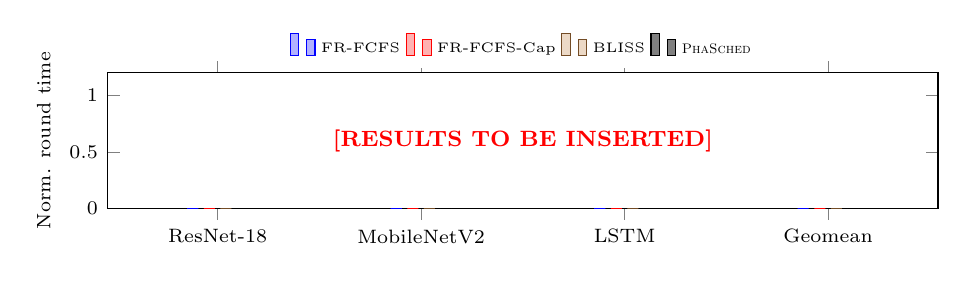
\begin{tikzpicture}
\begin{axis}[ybar,width=\columnwidth,height=3.3cm,ymin=0,ymax=1.2,
  ylabel={Norm. round time},ylabel style={font=\scriptsize},
  symbolic x coords={ResNet-18,MobileNetV2,LSTM,Geomean},xtick=data,
  tick label style={font=\scriptsize},enlarge x limits=0.18,bar width=4pt,
  legend style={font=\tiny,at={(0.5,1.03)},anchor=south,legend columns=4,draw=none}]
% Replace the zeros with measured values (normalised to FR-FCFS).
\addplot coordinates {(ResNet-18,0) (MobileNetV2,0) (LSTM,0) (Geomean,0)};
\addplot coordinates {(ResNet-18,0) (MobileNetV2,0) (LSTM,0) (Geomean,0)};
\addplot coordinates {(ResNet-18,0) (MobileNetV2,0) (LSTM,0) (Geomean,0)};
\addplot coordinates {(ResNet-18,0) (MobileNetV2,0) (LSTM,0) (Geomean,0)};
\legend{FR-FCFS,FR-FCFS-Cap,BLISS,\name{}}
\node[red,font=\footnotesize\bfseries] at (rel axis cs:0.5,0.5) {[RESULTS TO BE INSERTED]};
\end{axis}
\end{tikzpicture}
\caption{Round time normalised to FR-FCFS (lower is better).}
\label{fig:results}
\end{figure}

\section{Conclusion and Ongoing Work}
An FL round tells the system in advance what its memory traffic will look like. \name{} passes this knowledge to the memory controller with a 2-bit hint and re-tunes existing FR-FCFS knobs per phase. We are extending the study to asynchronous FL, where phases overlap, and to predicting the phase inside the controller from the read/write mix so that no software hint is required.

\bibliographystyle{IEEEtran}
\bibliography{refs}
\end{document}
